\documentclass{article}
\usepackage{tikz}
\usetikzlibrary{arrows.meta,positioning,calc,shapes.geometric}
\pagestyle{empty}
\begin{document}
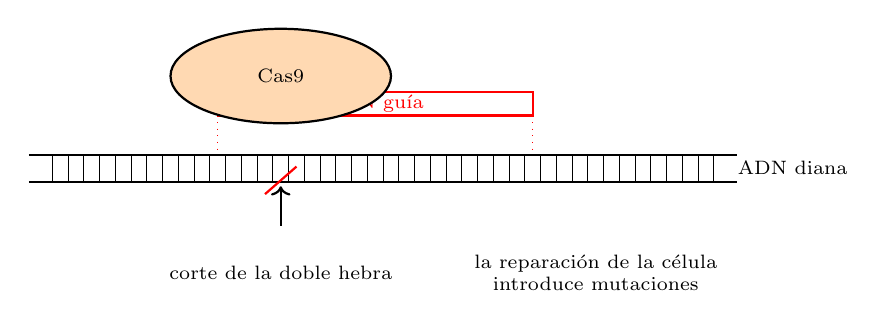
\begin{tikzpicture}
\tikzset{every node/.append style={align=center}}

\draw[thick] (0,0) -- (9,0); \draw[thick] (0,-0.35) -- (9,-0.35);
\foreach \x in {0.3,0.5,...,8.7} {\draw (\x,0) -- (\x,-0.35);}
\node[font=\scriptsize] at (9.7,-0.17) {ADN diana};
\draw[thick, red] (2.4,0.5) -- (6.4,0.5) -- (6.4,0.8) -- (2.4,0.8) -- cycle; \node[font=\scriptsize, red] at (4.4,0.65) {ARN guía};
\draw[dotted, red] (2.4,0.5) -- (2.4,0); \draw[dotted, red] (6.4,0.5) -- (6.4,0);
\draw[thick, fill=orange!30] (3.2,1.0) ellipse (1.4 and 0.6) node[font=\scriptsize] {Cas9};
\draw[->, thick] (3.2,-0.9) -- (3.2,-0.4); \draw[thick, red] (3.0,-0.5) -- (3.4,-0.15); 
\node[font=\scriptsize, align=center] at (3.2,-1.5) {corte de la doble hebra};
\node[font=\scriptsize, align=center] at (7.2,-1.5) {la reparación de la célula\\ introduce mutaciones};

\end{tikzpicture}
\end{document}
